
\begin{frame}{Modelling cooperativity}
\begin{columns}
\begin{column}{0.4\textwidth}
% For the simple case of a single transcription factor regulating the transcription rate of a single gene, the number of protein molecules produced of the regulated gene per unit time is a function of the concentration of the transcription factor in its active form~\cite{Alon2006}.
% The Hill equations~(\autoref{eq:Hill}) describe the cooperativity of binding for ligands to a receptor or for a similar binding event, for instance the binding of TFs to a regulatory region of DNA. The Hill equation is given here for the case of a single activator~(\autoref{eq:Hill_activator}) and a single repressor~(\autoref{eq:Hill_repressor}).
Single transcription factor regulating a single gene~\cite{Alon2006}
\begin{subequations}
\label{eq:Hill}
\begin{align}
\label{eq:Hill_activator}
\theta_{\text{activator}} &= \frac{p_j^{\nu_j}}{k_j^{\nu_j} + p_j^{\nu_j}} = \frac{\chi_j}{1 + \chi_j}
\\
\label{eq:Hill_repressor}
\theta_{\text{repressor}} &= \frac{1}{1 + \left(\frac{p_j}{k_j} \right)^{\nu_j}} = \frac{1}{1 + \chi_j}
\\
\chi_j &=
\left( \frac{p_j}{k_j} \right) ^ {\nu_j}
\end{align}
\end{subequations}
% Here $p_j$ is the ligand concentration (concentration of the $j$-th protein), $k_j$ and $\nu_j$ are model parameters. Different values for $k_j$ and the Hill coefficient $\nu_j$ determines $\theta$, which is the fraction of maximum transcription if regulated by either a single activator or repressor. If the concentration of ligand is $p_j = k_j$ then there will be half occupancy of the receptor. The basic assumption is that we use the fraction of occupancy of bound receptor~(the promotor of a gene), to describe transcription rate. The equations are sometimes multiplied by a constant $r_\text{max}$, which holds the maximum transcription rate unique to a given gene. This way $\theta$ will be the absolute instead of relative transcription rate, and have the dimension of $r_\text{max}$ instead of being dimensionless.


\end{column}
\begin{column}{0.6\textwidth}
\begin{figure}[ht]
\centering
\begin{subfigure}[b]{0.49\textwidth}\centering\caption{}
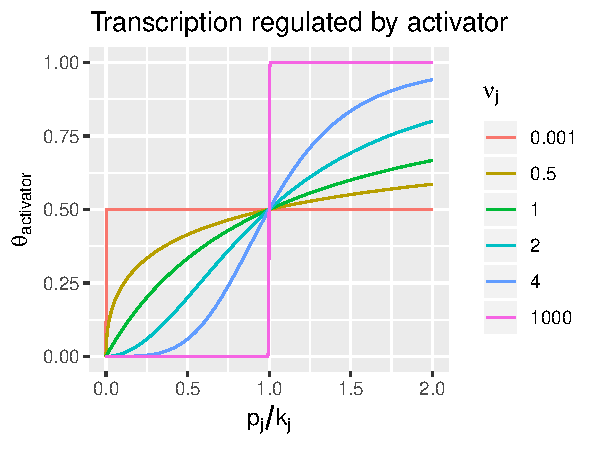
\includegraphics[width=\textwidth]{theory/fig/hill_activator.pdf}
\end{subfigure}
% \vskip\baselineskip
\begin{subfigure}[b]{0.49\textwidth}\centering\caption{}
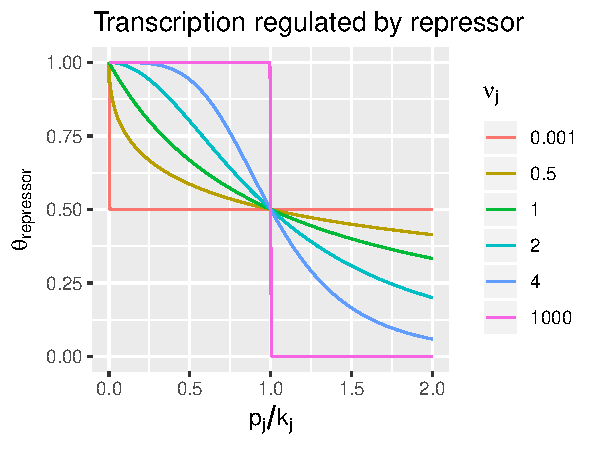
\includegraphics[width=\textwidth]{theory/fig/hill_repressor.pdf}
\end{subfigure}
\caption{\textbf{Hill equation models of gene regulation.} Single activator~(a), and repressor~(b).
% Unique curves result from using different model parameters $\nu_j$. 
}
\label{fig:Hill}
\end{figure}
% The equations are designed to capture cooperation in ligand binding as well as a receptor becoming saturated with increased ligand concentration~(\autoref{fig:Hill}).
% $\nu_j=1$ means that the receptor gets saturated linearly, $\nu_j<1$ means negative cooperation where it is more resistant to binding of ligand if some is already bound, and $\nu_j>1$ is positive cooperation. 
\end{column}
\end{columns}
\end{frame}

